\documentclass{article}
\usepackage[utf8]{inputenc}

\title{Comparing House Prices in Different Neighborhoods of Toronot, Canada}
\author{Edison Murairi }
\date{June 2020}

\usepackage{natbib}
\usepackage{graphicx}

\begin{document}

\maketitle

\section{Introduction}
\subsection{Background}
Toronto will experience a rapid population growth over the next 20 years. Even worse, this growth is accelerating, and is expected to double by the year 2041 \cite{toronto}. This rapid increase in the population number significantly affects the real estate in Toronto, leaving the low-income households most vulnerable to inadequate housings or to a lack of any at all. \\

This challenge requires that the real estate industry adaptates  to the economic conditions of every social class in Toronto. Otherwise, it will not provide profitable and comprehensive service to meet this challenge. The first to do this is to understand the current real estate conditions in Toronto. Therefore, in this project, we will compare the house prices in neighborhoods of Toronto. \\

As this challenge will surely affect various areas - urban planning, environment, finance, etc. - the findings are intended to multiple stakeholders. These stakeholders who will benefit from these findings are the urban planning office of the Canadian government, the Ministery of environment, and also the real estate companies operating in the country.

\subsection{Problem Statement}
How does the price of houses vary between different neighborhoods of Toronto?

\subsection{Data}
This project requires first the housing price data. We have obtained house sales data of the Province Ontario \cite{houses_sale}. This dataset contains 6 columns: address, areaName (the name of the area where the house is located), the price, the latitude and longitude of the location. Furthermore, there is no missing entry in the dataset. Figure \ref{fig:hs} shows an example of the house sales data.\\

\begin{figure}
	
	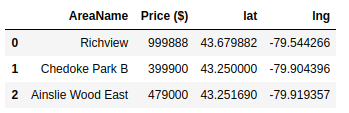
\includegraphics[]{hs.png}
	\caption{House Sales in the Ontario Province}
	\label{fig:hs}
	
\end{figure}

Secondly, we obtain venues data of each neighborhood from Foursquare using the postal codes obtained from the wikipedia page: "List of all Postal Codes in Canada M". From the Foursquare venues data, we will extract the neighborhood, the neighborhood latitude, the neighborhood longitude, the name of the venue, and the coordinates of the the venue (latitude and longitude)	Venue and the category of the venue. We will combine these informations with the the house sales data to compare how the price varies between neighborhoods of different characteristics. Figure \ref{fig:tv} shows an example of the venues data from Foursquare.

\begin{figure}[hbt!]
	
	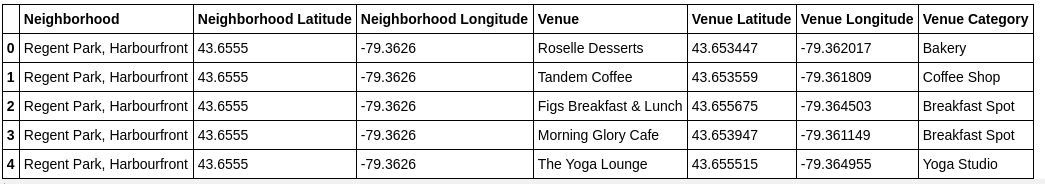
\includegraphics[width=\textwidth]{tv.png}
	\caption{Venues data in Toronto}
	\label{fig:tv}
	
\end{figure}




\bibliographystyle{plain}
\bibliography{references}
\end{document}
